% !TEX root =../main.tex
\chapter{Estimador PX4}\label{chp-01}

\lettrine[lraise=-0.1, lines=2, loversize=0.2]{E}{n} muchas ocasiones se tienen sensores con un retraso y una frecuencia de actualización muy diferentes entre ellos, por ejemplo una IMU es mucho más rápida que el procesamiento de la imagen de una cámara. PX4 lo soluciona añadiendo más elementos a la estructura original de un estimador de estados. Uno de los elementos es un \textit{Filtro de Kalman Extendido} (EKF). Este no usa las medidas más nuevas que le llegan, si no que las almacena y utiliza las que llegaron hace un determinado tiempo. Corriendo en paralelo pero a una frecuencia mayor, existe un estimador llamado \textit{Filtro de Salida}, el cual sí que utiliza la última medida del acelerómetro y del giróscopo. 

\section{Ejemplo}
Supongamos que se tiene un sistema que se mueve en el espacio del que se quiere conocer sus estados, en concreto, su posición, su velocidad y su ángulo. Para este objetivo se disponen de sensores que son: acelerómetro, giróscopo, GNSS y posición por visión. Cada uno de ellos tiene diferentes propiedades en cuanto a retraso, ruido, etc. que se muestran en la siguiente tabla. Se puede notar que la posición por visión es una fuente muy precisa de posición, pero sin embargo tiene un gran retraso desde que se toma la imagen hasta que se procesa, como suele suceder en la práctica. 
\begin{tabular}{|c|c|c|}
Sensor			& Retraso (ms) 	& Ruido 	\\ \hline 
acelerómetro 		& 0 		& 	      	\\ 
giróscopo 		& 0 		& 	      	\\ 
GNSS      		& 		& 	      	\\ % eliminar? 
Posición por visión 	& 30 		& 0.03 	
% Flujo óptico?
\end{tabular}

% EKF

En el primera ejecución del estimador, después de inicializar los estados, se toma una medida de la IMU (acelerómetro y giróscopo). El EKF todavía no la utiliza, si no que la guarda en su buffer. Conforme llegan nuevas medidas, las que ya estaban en el buffer se van desplazando hacia la derecha, hasta que llegan a la última celda y entonces son usadas por el EKF para estimar los estados. Estos estados y las medidas utilizadas para estimarlos se refieren al \textit{horizonte de tiempo retrasado}. 

% llega medida de visión
Pasan algunos ciclos más hasta que en el instante 40ms llega la primera medida de la visión, pero esta no se coloca junto con las medidas más recientes de la IMU, si no que se lleva directamenta a la última celda. En esta se encuentran también las medidas de la IMU tomadas en el instante 10ms, es decir hace 30 ms que coincide con el retraso que tiene la posición visual con respecto a la IMU. De esta manera se agrupan las medidas que se refieren al mismo instante físico, es decir, el instante en el que llegaron compensandose su retraso. 
\\
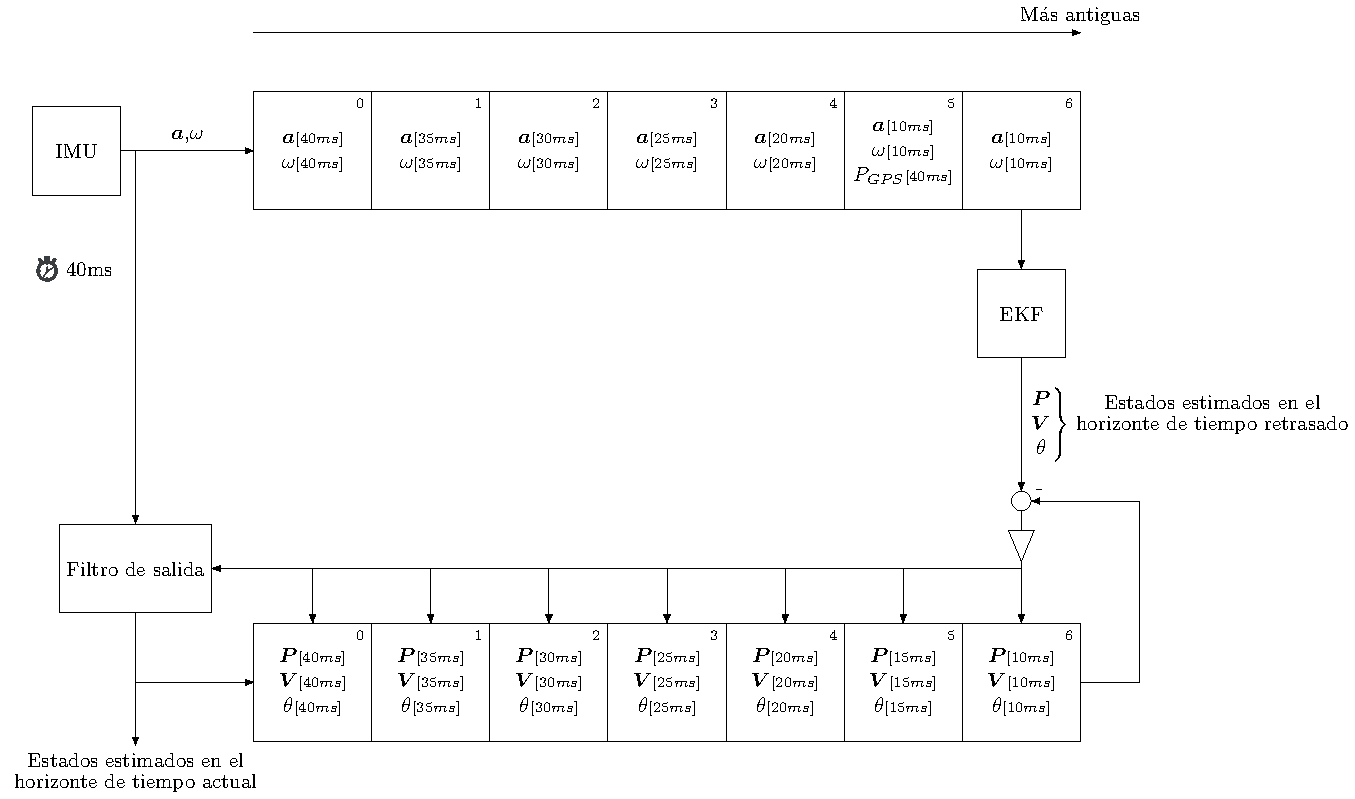
\includegraphics[width=\textwidth]{estimador_px4/tikz/ekf_output}


% Filtro de salida

De forma paralela se ejecuta el \textit{filtro de salida} que solamente utiliza las medidas de la IMU, en este caso las que se generan más recientemente.
Los estados de este último filtro, la posición, velocidad y orientación,  se han estado guardando en el \textit{buffer de salida}.  
De este buffer se cogen los estados más antiguos y se compara con los estados generados por EKF. Su diferencia se multiplica por una ganancia se le suma a todos los elementos del buffer de salida.  

\subsection{Detalles de implementación}
\begin{itemize}
\item La ganancia que multiplica la diferencia entre el filtro de salida y el EKF y que sirve para corregir los estados, se calcula de manera el sistema controlado tenga un factor de amortiguamiento de 0.7
\begin{equation}
K_p=\frac{0.5}{Retraso}
\end{equation} 
{\color{red} Buscar la deducción hasta esta expresión}
\end{itemize}
\section{EKF para modelo bidimensional}
Se va aplicar a un quadrotor en 2 dimensiones, pero el modelo al no ser dinámico, se podria aplicar a cualquier otro móvil.

Estados:
\begin{align}
X = 
\begin{bmatrix} 
x \\ y \\ V_x \\ V_y \\ \theta
\end{bmatrix}
\end{align}

Modelo de predicción (modelo cinemático, no dinámico):
\begin{align}
\begin{bmatrix} 
x \\ y 
\end{bmatrix}_{k+1}
=
\begin{bmatrix} 
x \\ y 
\end{bmatrix}_k
+
\begin{bmatrix} 
V_x \\ V_y 
\end{bmatrix}_k
\Delta t
\end{align}

\begin{align}
\begin{bmatrix} 
V_x \\ V_y 
\end{bmatrix}_{k+1}
=
\begin{bmatrix} 
V_x \\ V_y 
\end{bmatrix}_k + 
\Delta t
\begin{bmatrix} 
\cos{\theta} & \sin{\theta} \\ -\sin{\theta} & \cos{\theta}
\end{bmatrix}
\bm{a} +  
\begin{bmatrix} 
0 \\ - m\ g 
\end{bmatrix}\Delta t
\end{align}

\begin{align}
\theta_{k+1} = \theta_k + \Delta t \omega
\end{align}


Jacobiano del modelo de predicción:
\begin{align}
F = 
\begin{bmatrix} 
%x/X
1 	&0	&\Delta t	&0		&0\\
%y/X
0 	&1	&0		&\Delta t	&0\\
%Vx/X
0 	&0	&1		&0		&\Delta t\left(-a_x\sin{\theta} + a_y\cos{\theta}\right) \\
%Vy/X
0 	&0	&0		&1		&\Delta t\left(-a_x\cos{\theta} - a_y\sin{\theta}\right) \\
%theta/X
0 	&0	&0		&0		&1
\end{bmatrix}
\end{align}

Jacobiano del acelerómetro y el giróscopo
\begin{align}
G = 
\begin{bmatrix} 
%x/a,w
0 			&0			&0\\
%y/a,w
0 			&0			&0\\
%Vx/a,w
\Delta t \cos{\theta} 	&\Delta t \sin{\theta}	&0\\
%Vy/a,w
-\Delta t \sin{\theta} 	&\Delta t \cos{\theta}	&0\\
%theta/a,w
0 			&0			&1		
\end{bmatrix}
\end{align}

Matriz de covarianzas de la predicción:
\begin{align}
Q = 
G
\begin{bmatrix} 
\sigma^2_a 	& 0 		& 0\\
0 		& \sigma^2_a 	& 0\\
0 		& 0 		& \sigma^2_\omega\\
\end{bmatrix}
G^T
\end{align}


\endinput
